\documentclass[9pt]{beamer}
\mode<presentation>
\usepackage[T1]{fontenc}
\usepackage{color}
\usepackage{graphicx}
\usepackage{natbib}
\usepackage{tikz}
\usetikzlibrary{shapes.geometric}
\usepackage{xmpmulti}
\usepackage{animate}
\usepackage{tcolorbox}
\usepackage{amsmath}
\usepackage{gensymb}
\usepackage{csquotes}
\usepackage{bibentry}
\nobibliography*

%\usetheme{Singapore}

\setbeamercolor{block title}{bg=structure!20}
\setbeamercolor{block body}{bg=structure!10}
\setbeamertemplate{blocks}[rounded][shadow]
%\usecolortheme{seahorse}

\usefonttheme{professionalfonts}

\title[Climate Impacts]{Machine learning-based evidence and attribution mapping of 100,000 climate impact studies}
\author{Max Callaghan, Carl-Friedrich Schleussner, Shruti Nath, Gerrit Hansen, Quentin Lejeune, Tom Knutson, Markus Reichstein, Emily Theokritoff, Marina Andrijevic, Robert Brecha, Michael Hegarty, Chelsea Jones, Kaylin Lee, Agathe Lucas, Nicole van Maanen, Inga Menke, Peter Pfleiderer, Burcu Yesil, Jan Minx }
\institute[MCC]{
	\includegraphics[height=1cm,width=2cm]{images/MCC_Logo_RZ_rgb.jpg} \hspace{5em} \includegraphics[height=1cm]{images/climate_analytics.png}
}
\date{}
\newif\ifframeinlbf
\frameinlbftrue
\makeatletter
\newcommand\listofframes{\@starttoc{lbf}}
\makeatother

\addtobeamertemplate{frametitle}{}{%
	\ifframeinlbf
	\addcontentsline{lbf}{section}{\protect\makebox[2em][l]{%
			\protect\usebeamercolor[fg]{structure}\insertframenumber\hfill}%
		\insertframetitle\par}%
	\else\fi
}

\newtheorem*{remark}{}

\bibliographystyle{apalike}

\begin{document}
	
\begin{frame}
	\titlepage
\end{frame}


%%%%%%%%%%%%%%%%%%%%%%%%%%%%%%%%%%%%%%%%%%%%%%%%%%
%% Introduction
\section{Introduction}

%\begin{frame}
%\tableofcontents[currentsection]
%\end{frame}

\begin{frame}{Context}

Systematic assessments of the evidence on Climate Change like those conducted by the IPCC are vital.

\begin{columns}
	\begin{column}{0.618\linewidth}
		\begin{figure}
			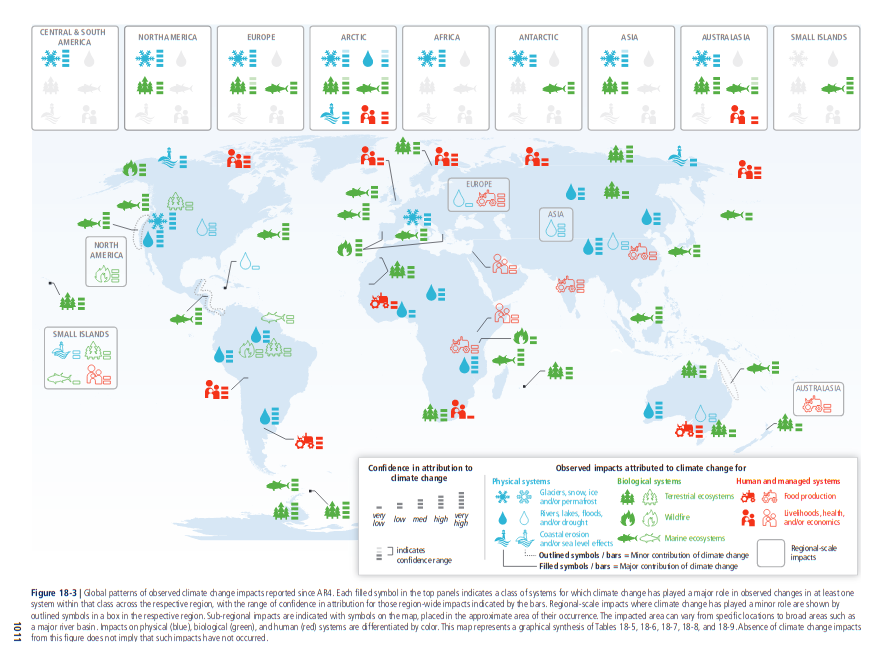
\includegraphics[width=\linewidth]{images/map_18.png}<1->
		\end{figure}
	\end{column}
	\begin{column}{0.312\linewidth}
		
		\begin{figure}
			\includegraphics[width=\linewidth]{images/pubs_time_wgb_lp.pdf}<2->
		\end{figure}
		
		\begin{itemize}
			\small
			\item<2->These are challenged by big literature \cite{Callaghan2020} 
			\item<3->They do not account for uncertainty about what literature is available
		\end{itemize}
	\end{column}
\end{columns}

\end{frame}

%\begin{frame}{Quantifying the literature}
%
%\begin{columns}
%	
%	\begin{column}{0.382\linewidth}
%	\begin{itemize}
%		\item AR5 WGII started with a basic bibliometric analysis of climate change (and impacts and adaptation) literature
%		\item The literature has doubled again since then
%		\item We can do more than this
%	\end{itemize}
%\end{column}
%
%	\begin{column}{0.618\linewidth}
%		\begin{figure}
%			\includegraphics[width=0.7\textheight]{ar5_fig_1_1}
%		\end{figure}
%	\end{column}
%
%\end{columns}
%
%\end{frame}


\begin{frame}{Process}

\begin{enumerate}
	\item Broad \textbf{search} in literature databases (Web of Science \& Scopus) for literature on climate impacts
	\item Hand \textbf{screen and code} documents to include only documents on observed climate impacts, and code the type of impacts and type of evidence
	\item Combine this training data with the categorisation of documents in \textbf{AR5}
	\item Use supervised \textbf{machine learning} to predict the inclusion and impact type of 100s of thousands or remaining documents
	\item Use named entity recognition to extract \textbf{geographical locations} from titles and abstracts
	\item Map entities to grid cells and combine with \textbf{WGI style D\&A} of temperature and precipitation trends at the grid cell level
	\item Describe \textbf{evidence gluts and gaps} at a grid cell level
	
\end{enumerate}

\end{frame}

\begin{frame}{Process}
\begin{figure}
	\includegraphics[width=0.65\linewidth]{../figures/process.pdf}
\end{figure}
\end{frame}

\begin{frame}{Questions for CVM}
\large
\begin{itemize}
	\item How to aggregate, how to merge (w.r.t space and time and content) with other data?
	\item What documents to include?
	\item At what level do we want to categorise impact type?
	\item Can we screen more documents to improve predictions?
\end{itemize}
\end{frame}

\begin{frame}{Search query I}

We built a query using the documents from the tables in AR5 WGII Chapter 18.

The ideal query should contain \textit{all} documents included in those tables, along with \textit{all} additional relevant documents (untestable) and a hopefully minimal amount of irrelevant documents

\begin{figure}
	\includegraphics[width=0.7\linewidth]{../plots/basic_lit_plot.png}<1>
	\includegraphics[width=0.7\linewidth]{../plots/lit_plot_query_1.png}<2>
	\includegraphics[width=0.7\linewidth]{../plots/lit_plot_query_3.png}<3>
	\includegraphics[width=0.7\linewidth]{../plots/lit_plot_query_2.png}<4>
\end{figure}
\end{frame}

\begin{frame}{Search query II}

Our query contained a list of climate variables, a list of impacts, and a list of words narrowing down the literature on observed impacts

\begin{columns}
\begin{column}{0.33\linewidth}
	\textbf{Climate}
	
	\scriptsize
	
	TS=("climate model" OR "elevated* temperatur" OR "ocean* warming" OR "saline* intrusion" OR "chang* climat" OR "environment* change" OR "climat* change" OR "climat* warm" OR "warming* climat" OR "climat* varia" OR "global* warming" OR "global* change" OR "greenhouse* effect" OR "snow cover" OR "extreme temperature" OR "cyclone" OR "ocean acidification" OR "anthropogen*" OR "sea* level" OR "precipitation variabil*" OR "precipitation change*" OR "temperature* impact" OR "environmental* variab" OR "weather* pattern" OR "weather* factor*" OR "climat*") OR TS=("change* NEAR/5 cryosphere" OR "increase* NEAR/3 temperatur*")) 
	
\end{column}
\begin{column}{0.33\linewidth}
	
	\textbf{Impacts}
	
	\scriptsize
	
	AND (TS=("migration" OR "impact*" OR "specie*" OR "mortality*" OR "health" OR "disease*" OR "ecosystem*" OR "mass balance" OR "flood*" OR "drought" OR "disease*" OR "adaptation" OR "malaria" OR "fire" OR "water scarcity" OR "water supply" OR "permafrost" OR "biological response" OR "food availability" OR "food security" OR "vegetation dynamic*" OR "cyclone*" OR "yield*" OR "gender" OR "indigenous" OR "conflict" OR "inequality" OR "snow water equival*" OR "surface temp*") OR TS=("glacier* NEAR/3 melt*" OR "glacier* NEAR/3 mass*" OR "erosion* NEAR/5 coast*" OR "glacier* NEAR/5 retreat*" OR "rainfall* NEAR/5 reduc*" OR "coral* NEAR/5 stress*" OR "precip* NEAR/5 *crease*" OR "river NEAR/5 flow"))
	
\end{column}
\begin{column}{0.33\linewidth}
	
	\textbf{Observed}
	
	\scriptsize
	
	AND (TS=("recent" OR "current" OR "modern" OR "observ*" OR "evidence*" OR "past" OR "local" OR "region*" OR "significant" OR "driver*" OR "driving” OR "respon*" OR "were responsible" OR "was responsible" OR "exhibited" OR "witnessed" OR "attribut*" OR "has increased" OR "has decreased" OR "histor*" OR "correlation" OR "evaluation") )
\end{column}	
\end{columns}

\end{frame}

\begin{frame}{Screening \& Labelling}

\begin{figure}
	\includegraphics[width=\linewidth]{../plots/screening-platform}
\end{figure}

\end{frame}



%%%%%%%%%%%%%%%%%%%%%%%%%%%%%%%%%%%%%%%%%%%%%%%%%%
%% Machine learning
\section{Machine learning}

\begin{frame}{Basic ML I - text as data}

We can build a set of features is from a TFIDF weighted set of unigrams and bigrams from the documents' abstracts

\medskip

\begin{columns}
	\begin{column}{0.5\linewidth}
		\includegraphics[width=\linewidth]{images/doc_example.png}
	\end{column}
	\begin{column}{0.5\linewidth}
		\includegraphics[width=\linewidth]{images/example_doc_tfidf.pdf}
	\end{column}
\end{columns}

\medskip

We discard very uncommon and very common features, leaving us with a vocabulary of 7,394 unique features.

\end{frame}

\begin{frame}{Basic ML II - Support Vector Machines}

SVMs try to fit a hyperplane through the multidimensional feature space (represented below in 2D) that best separates the classes in the training data.

\begin{columns}
\begin{column}{0.618\linewidth}
	\begin{figure}
		\includegraphics[width=\linewidth]{images/svc_sklearn_unbalanced.png}
	\end{figure}
\end{column}
\begin{column}{0.382\linewidth}
	With SVMs we ignore word order and context (bag of words assumption).
\end{column}
\end{columns}

\end{frame}



\begin{frame}{Fancy ML I - BERT}

BERT (Bidirectional Representations from Transformers) is trained (by Google) on huge text corpora, and can be \textbf{``fine tuned''} on custom tasks. 

\begin{figure}
	\includegraphics[width=\linewidth]{images/bert-transfer-learning.png}
	\caption{Source: \url{https://jalammar.github.io/illustrated-bert/}}
\end{figure}

\end{frame}

\begin{frame}{Fancy ML II - Masked Language Modelling}

BERT is trained by feeding it millions of sentences from Wikipedia etc. and asking it to predict missing words.

\begin{columns}
	\begin{column}{0.618\linewidth}
		\begin{figure}
			\includegraphics[width=\linewidth]{images/BERT-language-modeling-masked-lm.png}
			\caption{Source: \url{https://jalammar.github.io/illustrated-bert/}}
		\end{figure}
	\end{column}
	\begin{column}{0.382\linewidth}
		The model is trained on this task in two directions (left to right and right to left) - hence Bidirectional.
		
		\medskip
		
		This generates embeddings (representations of words as vectors) which are contextually aware.
	\end{column}
\end{columns}

\end{frame}


\begin{frame}{ML I - Training and Validation}

\small

You can assess a model by \textbf{training} it on one subset of data, and \textbf{testing} it on another. Models have different settings (hyperparameters) that affect how well they perform on a given dataset. Separating hyperparameter optimisation from performance estimation prevents overfitting, hence \textbf{nested cross-validation}.
		
\begin{columns}
	\begin{column}{0.618\linewidth}
	\begin{figure}
		\includegraphics[width=\linewidth]{../figures/si_figure_2.pdf}
	\end{figure}
	\end{column}

	\begin{column}{0.382\linewidth}
		\begin{itemize}
			\item In the inner loop, a model is trained on \textbf{Inner train} and tested on \textbf{Inner validation} with each combination of hyperparameters. 
			\item The best performing model is selected and then trained on the outer \textbf{Train} and tested on the outer \textbf{Test}. 
			\item For the final model used to make predictions, each candidate is tested in each outer loop and the best performing is selected.
		\end{itemize}

	\end{column}
\end{columns}

\medskip

This process validates the \textbf{hyperparameter optimisation procedure} itself, rather than a specific set of hyperparameters. The estimation of performance is more generalisable.

\end{frame}

\begin{frame}{ML II - results}

BERT outperformed SVM by all performance metrics

\begin{figure}
	\includegraphics[width=\linewidth]{../figures/SI_figure_3.pdf}
\end{figure}

\end{frame}

\begin{frame}{ML II - results II}

BERT outperformed SVM by all performance metrics

\begin{columns}
	\begin{column}{0.618\linewidth}
		\begin{figure}
			\includegraphics[width=\linewidth]{../figures/SI_figure_4.pdf}
		\end{figure}
	\end{column}
	
	\begin{column}{0.382\linewidth}
			Performance of impact type classifier higher than classifier for inclusion (provides evidence of observed impacts of climate change)
	\end{column}
\end{columns}



\end{frame}

\begin{frame}{Results}

\begin{columns}
	\begin{column}{0.618\linewidth}
		\begin{figure}
			\includegraphics[width=\linewidth]{../figures/figure_1.png}
		\end{figure}
	\end{column}
	\begin{column}{0.382\linewidth}
		\begin{itemize}
			\item We identify nearly 100,000 documents likely to be relevant
			\item We predict impact type, and extract locations
		\end{itemize}
	
	\end{column}
\end{columns}

\end{frame}

%%%%%%%%%%%%%%%%%%%%%%%%%%%%%%%%%%%%%%%%%%%%%%
%% D&A


\begin{frame}{Synthesizing impacts evidence with quantitative detection and attribution evidence}

We know from detection and attribution studies whether observed trends in temperature and precipitation are attributable to human influence on the climate.

\cite{Knutson2013, Knutson2018} show this on a grid cell level

\begin{columns}
	\begin{column}{0.65\linewidth}
		\includegraphics[width=\linewidth]{images/knutson_precip_da}
	\end{column}
	\begin{column}{0.35\linewidth}
		\includegraphics[width=\linewidth]{images/knutson_temp_da}
	\end{column}
\end{columns}

We update these calculations and combine with information from our database of impacts evidence, in which the locations, and the climate drivers have been predicted

\end{frame}

\begin{frame}{Synthesising impacts with D\&A evidence}

\small

\begin{columns}
	\begin{column}{0.6\linewidth}
		\begin{figure}
			\includegraphics[width=\linewidth]{../figures/si_figure_9.pdf}
		\end{figure}
	\end{column}
	\begin{column}{0.4\linewidth}
		\begin{itemize}
			\item 20 out of 27 gridcells in Sudan display an attributable increase in temperature
			\item So each study referring to Sudan refers to a place where around 74\% of the gridcells display attributable increases in temp.
		\end{itemize}
				\rule{\linewidth}{0.2pt}
		\begin{itemize}
			\item 11 studies refer to Sudan (as the smallest identifiable geographical entity), and Sudan has 27 gridcells
			\item We apportion these studies to the relevant gridcells, calculating that each gridcell in Sudan has $\frac{11}{27}$ studies referring to it
			\item We do the same for each further geographical entity
		\end{itemize}
		
	\end{column}
\end{columns}

\end{frame}


\begin{frame}{We combine all this information to show evidence gaps and gluts}

\begin{columns}
	\begin{column}{0.9\linewidth}
		\begin{figure}
			\includegraphics[width=\linewidth]{../figures/figure_2.png}
		\end{figure}
	\end{column}
\end{columns}

\end{frame}

\begin{frame}{Conclusions}

\begin{itemize}
	\item We identify a large body of evidence about climate impacts, emphasising what we have seen recently: we are already feeling the effects of climate change
	\item What we know about the effects of a changing climate on human and natural systems does not always match with what we know about how (and where) humans are driving changes in climate variables:
	\begin{itemize}
		\item In high income countries, 88\%5 population live in areas with attributable climate changes and high evidence of the impacts of those changes in human and natural systems
		\item In low income countries, 74\% of population live in areas with attributable climate changes, but for almost a third of that population, there low evidence of the impacts of those changes -> \textbf{attribution gap}
	\end{itemize}
\end{itemize}

\textbf{But}, 

\begin{itemize}
	\item Current results only show studies in Web of Science and scopus, so definitely do not show all relevant studies
	\item Although our query returned all papers in the relevant AR5 section, it may still miss potentially relevant literature.
	\item Study identification is approximate and uncertain, trends in studies may not correspond to trends attributed to human influence
	\item Geoparsing is also inexact, and is unable to grasp fuzzy geographical content e.g. "Western China"
\end{itemize}

\end{frame}

\begin{frame}{Summary - Machine learning-based evidence and attribution mapping of 100,000 climate impact studies}

\begin{columns}
	\small
	\begin{column}{0.5\linewidth}
		\begin{itemize}
			\item In a large collaborative coding exercise, we examined thousands of papers \textit{potentially} relevant to understanding observed impacts of climate change
			\item We used machine learning to identify tens > 100,000 studies \textit{likely} to be relevant.
			\item We predicted the sector, climate driver, and location for each of these studies
			\item We used the location and predicted climate driver to synthesise this information with existing quantitative Detection and Attribution knowledge.
		\end{itemize}
	\end{column}

	\begin{column}{0.5\linewidth}
		
		\begin{block}{Takeaways}
			\begin{itemize}
				\item Machine learning can inform and support global environmental assessments
				\item We have lots of evidence of observed impacts of climate change, on all continents and in all systems.
				\item What we know about the effects of a changing climate on human and natural systems does not always match with what we know about how (and where) humans are driving changes in climate variables 
			\end{itemize}
		\end{block}
		
	\end{column}
\end{columns}



\begin{center}
	\line(1,0){250}
	
	\medskip
	
	\textbf{Thanks!}
	
	\medskip
	
	Contact: \url{callaghan@mcc-berlin.net}

\end{center}



\end{frame}

%%%%%%%%%%%%
%% Bib
\begin{frame}{Bibliography}
\bibliography{../mendeley}
\end{frame}

\end{document}